
\documentclass[letterpaper,hide notes,xcolor={table,svgnames},pdftex,10pt]{beamer}
\def\showexamples{t}


%\usepackage[svgnames]{xcolor}

%% Demo talk
%\documentclass[letterpaper,notes=show]{beamer}

\usecolortheme{crane}
\setbeamertemplate{navigation symbols}{}

\usetheme{MyPittsburgh}
%\usetheme{Frankfurt}

%\usepackage{tipa}

\usepackage{hyperref}
\usepackage{graphicx,xspace}
\usepackage[normalem]{ulem}
\usepackage{multicol}
\usepackage{amsmath,amssymb,amsthm,graphicx,xspace}
\newcommand\SF[1]{$\bigstar$\footnote{SF: #1}}

\usepackage[default]{sourcesanspro}
\usepackage[T1]{fontenc}

\newcounter{tmpnumSlide}
\newcounter{tmpnumNote}

% old question code
%\newcommand\question[1]{{$\bigstar$ \small \onlySlide{2}{#1}}}
% \newcommand\nquestion[1]{\ifdefined \presentationonly \textcircled{?} \fi \note{\par{\Large \textbf{?}} #1}}
% \newcommand\nanswer[1]{\note{\par{\Large \textbf{A}} #1}}


 \newcommand\mnote[1]{%
   \addtocounter{tmpnumSlide}{1}
   \ifdefined\showcues {~\tiny\fbox{\arabic{tmpnumSlide}}}\fi
   \note{\setlength{\parskip}{1ex}\addtocounter{tmpnumNote}{1}\textbf{\Large \arabic{tmpnumNote}:} {#1\par}}}

\newcommand\mmnote[1]{\note{\setlength{\parskip}{1ex}#1\par}}

%\newcommand\mnote[2][]{\ifdefined\handoutwithnotes {~\tiny\fbox{#1}}\fi
% \note{\setlength{\parskip}{1ex}\textbf{\Large #1:} #2\par}}

%\newcommand\mnote[2][]{{\tiny\fbox{#1}} \note{\setlength{\parskip}{1ex}\textbf{\Large #1:} #2\par}}

\newcommand\mquestion[2]{{~\color{red}\fbox{?}}\note{\setlength{\parskip}{1ex}\par{\Large \textbf{?}} #1} \note{\setlength{\parskip}{1ex}\par{\Large \textbf{A}} #2\par}\ifdefined \presentationonly \pause \fi}

\newcommand\blackboard[1]{%
\ifdefined   \showblackboard
  {#1}
  \else {\begin{center} \fbox{\colorbox{blue!30}{%
         \begin{minipage}{.95\linewidth}%
           \hspace{\stretch{1}} Some space intentionally left blank; done at the blackboard.%
         \end{minipage}}}\end{center}}%
         \fi%
}



%\newcommand\q{\tikz \node[thick,color=black,shape=circle]{?};}
%\newcommand\q{\ifdefined \presentationonly \textcircled{?} \fi}

\usepackage{listings}
\lstset{%
  keywordstyle=\bfseries,
  aboveskip=15pt,
  belowskip=15pt,
  captionpos=b,
  identifierstyle=\ttfamily,
  escapeinside={(*@}{@*)},
  stringstyle=\ttfamiliy,
  frame=lines,
  numbers=left, basicstyle=\scriptsize, numberstyle=\tiny, stepnumber=0, numbersep=2pt}

\usepackage{siunitx}
\newcommand\sius[1]{\num[group-separator = {,}]{#1}\si{\micro\second}}
\newcommand\sims[1]{\num[group-separator = {,}]{#1}\si{\milli\second}}
\newcommand\sins[1]{\num[group-separator = {,}]{#1}\si{\nano\second}}
\sisetup{group-separator = {,}, group-digits = true}

%% -------------------- tikz --------------------
\usepackage{tikz}
\usetikzlibrary{positioning}
\usetikzlibrary{arrows,backgrounds,automata,decorations.shapes,decorations.pathmorphing,decorations.markings,decorations.text}

\tikzstyle{place}=[circle,draw=blue!50,fill=blue!20,thick, inner sep=0pt,minimum size=6mm]
\tikzstyle{transition}=[rectangle,draw=black!50,fill=black!20,thick, inner sep=0pt,minimum size=4mm]

\tikzstyle{block}=[rectangle,draw=black, thick, inner sep=5pt]
\tikzstyle{bullet}=[circle,draw=black, fill=black, thin, inner sep=2pt]

\tikzstyle{pre}=[<-,shorten <=1pt,>=stealth',semithick]
\tikzstyle{post}=[->,shorten >=1pt,>=stealth',semithick]
\tikzstyle{bi}=[<->,shorten >=1pt,shorten <=1pt, >=stealth',semithick]

\tikzstyle{mut}=[-,>=stealth',semithick]

\tikzstyle{treereset}=[dashed,->, shorten >=1pt,>=stealth',thin]

\usepackage{ifmtarg}
\usepackage{xifthen}
\makeatletter
% new counter to now which frame it is within the sequence
\newcounter{multiframecounter}
% initialize buffer for previously used frame title
\gdef\lastframetitle{\textit{undefined}}
% new environment for a multi-frame
\newenvironment{multiframe}[1][]{%
\ifthenelse{\isempty{#1}}{%
% if no frame title was set via optional parameter,
% only increase sequence counter by 1
\addtocounter{multiframecounter}{1}%
}{%
% new frame title has been provided, thus
% reset sequence counter to 1 and buffer frame title for later use
\setcounter{multiframecounter}{1}%
\gdef\lastframetitle{#1}%
}%
% start conventional frame environment and
% automatically set frame title followed by sequence counter
\begin{frame}%
\frametitle{\lastframetitle~{\normalfont(\arabic{multiframecounter})}}%
}{%
\end{frame}%
}
\makeatother

\makeatletter
\newdimen\tu@tmpa%
\newdimen\ydiffl%
\newdimen\xdiffl%
\newcommand\ydiff[2]{%
    \coordinate (tmpnamea) at (#1);%
    \coordinate (tmpnameb) at (#2);%
    \pgfextracty{\tu@tmpa}{\pgfpointanchor{tmpnamea}{center}}%
    \pgfextracty{\ydiffl}{\pgfpointanchor{tmpnameb}{center}}%
    \advance\ydiffl by -\tu@tmpa%
}
\newcommand\xdiff[2]{%
    \coordinate (tmpnamea) at (#1);%
    \coordinate (tmpnameb) at (#2);%
    \pgfextractx{\tu@tmpa}{\pgfpointanchor{tmpnamea}{center}}%
    \pgfextractx{\xdiffl}{\pgfpointanchor{tmpnameb}{center}}%
    \advance\xdiffl by -\tu@tmpa%
}
\makeatother
\newcommand{\copyrightbox}[3][r]{%
\begin{tikzpicture}%
\node[inner sep=0pt,minimum size=2em](ciimage){#2};
\usefont{OT1}{phv}{n}{n}\fontsize{4}{4}\selectfont
\ydiff{ciimage.south}{ciimage.north}
\xdiff{ciimage.west}{ciimage.east}
\ifthenelse{\equal{#1}{r}}{%
\node[inner sep=0pt,right=1ex of ciimage.south east,anchor=north west,rotate=90]%
{\raggedleft\color{black!50}\parbox{\the\ydiffl}{\raggedright{}#3}};%
}{%
\ifthenelse{\equal{#1}{l}}{%
\node[inner sep=0pt,right=1ex of ciimage.south west,anchor=south west,rotate=90]%
{\raggedleft\color{black!50}\parbox{\the\ydiffl}{\raggedright{}#3}};%
}{%
\node[inner sep=0pt,below=1ex of ciimage.south west,anchor=north west]%
{\raggedleft\color{black!50}\parbox{\the\xdiffl}{\raggedright{}#3}};%
}
}
\end{tikzpicture}
}


%% --------------------

%\usepackage[excludeor]{everyhook}
%\PushPreHook{par}{\setbox0=\lastbox\llap{MUH}}\box0}

%\vspace*{\stretch{1}

%\setbox0=\lastbox \llap{\textbullet\enskip}\box0}

\setlength{\parskip}{\fill}

\newcommand\noskips{\setlength{\parskip}{1ex}}
\newcommand\doskips{\setlength{\parskip}{\fill}}

\newcommand\xx{\par\vspace*{\stretch{1}}\par}
\newcommand\xxs{\par\vspace*{2ex}\par}
\newcommand\tuple[1]{\langle #1 \rangle}
\newcommand\code[1]{{\sf \footnotesize #1}}
\newcommand\ex[1]{\uline{Example:} \ifdefined \presentationonly \pause \fi
  \ifdefined\showexamples#1\xspace\else{\uline{\hspace*{2cm}}}\fi}

\newcommand\ceil[1]{\lceil #1 \rceil}


\AtBeginSection[]
{
   \begin{frame}
       \frametitle{Outline}
       \tableofcontents[currentsection]
   \end{frame}
}



\pgfdeclarelayer{edgelayer}
\pgfdeclarelayer{nodelayer}
\pgfsetlayers{edgelayer,nodelayer,main}

\tikzstyle{none}=[inner sep=0pt]
\tikzstyle{rn}=[circle,fill=Red,draw=Black,line width=0.8 pt]
\tikzstyle{gn}=[circle,fill=Lime,draw=Black,line width=0.8 pt]
\tikzstyle{yn}=[circle,fill=Yellow,draw=Black,line width=0.8 pt]
\tikzstyle{empty}=[circle,fill=White,draw=Black]
\tikzstyle{bw} = [rectangle, draw, fill=blue!20, 
    text width=4em, text centered, rounded corners, minimum height=2em]
    
    \newcommand{\CcNote}[1]{% longname
	This work is licensed under the \textit{Creative Commons #1 3.0 License}.%
}
\newcommand{\CcImageBy}[1]{%
	\includegraphics[scale=#1]{creative_commons/cc_by_30.pdf}%
}
\newcommand{\CcImageSa}[1]{%
	\includegraphics[scale=#1]{creative_commons/cc_sa_30.pdf}%
}
\newcommand{\CcImageNc}[1]{%
	\includegraphics[scale=#1]{creative_commons/cc_nc_30.pdf}%
}
\newcommand{\CcGroupBySa}[2]{% zoom, gap
	\CcImageBy{#1}\hspace*{#2}\CcImageNc{#1}\hspace*{#2}\CcImageSa{#1}%
}
\newcommand{\CcLongnameByNcSa}{Attribution-NonCommercial-ShareAlike}

\newenvironment{changemargin}[1]{% 
  \begin{list}{}{% 
    \setlength{\topsep}{0pt}% 
    \setlength{\leftmargin}{#1}% 
    \setlength{\rightmargin}{1em}
    \setlength{\listparindent}{\parindent}% 
    \setlength{\itemindent}{\parindent}% 
    \setlength{\parsep}{\parskip}% 
  }% 
  \item[]}{\end{list}} 




\title{Lecture 9 --- Reduction to Relational Schema, Design Decisions}

\author{Jeff Zarnett \\ \small \texttt{jzarnett@uwaterloo.ca}}
\institute{Department of Electrical and Computer Engineering \\
  University of Waterloo}
\date{\today}


\begin{document}

\begin{frame}
  \titlepage

 \end{frame}



\begin{frame}
\frametitle{Modelling Diagrams into Tables}

If we have an entity-relation diagram, eventually we will want to turn that into a set of database tables. 

The conversion routine is not especially complicated. 

After a small amount of practice it is likely that you will be able to do it quickly and efficiently.

\end{frame}



\begin{frame}
\frametitle{Strong Entities}

Strong entities are the easiest to turn into tables. 

The name of the table will be the name of the entity (surprise) and the attributes in the diagram become the attributes in the relation. 

The primary key in the table will be the same as the primary key in the diagram. 


\end{frame}



\begin{frame}
\frametitle{Strong Entities}

If the diagram says an instructor has \textit{(id, name, salary)} and \textit{id} is the primary key:

The create table statement will assign types and lengths to these fields. 

\end{frame}



\begin{frame}
\frametitle{Weak Entities}

Suppose $A$ is a weak entity set and the strong attribute it depends on is $B$. 

The weak entity table is created using the attributes of $A$ as well as the primary key of $B$, the entity it depends upon. 

Suppose the weak entity is the section of a course, as before, and course is the strong entity. 

The section entity would be created with all attributes of the section (weak) entity and the primary key  of the course entity (course id).


\end{frame}




\begin{frame}
\frametitle{Weak Entities}

It is also sensible to add constraints to this table that says the attribute(s) referencing the primary key of the strong entity  must exist.

This means: not null and foreign key. 

In the weak entity table, the primary key is formed by the key referencing the strong entity plus the discriminator.

\end{frame}



\begin{frame}
\frametitle{Weak Entities}

Example: theweak entity is a list of something and the strong entity a container.

Suppose you have a shipment: a single shipment is made up of items and those items are, let's say, weak entities in the example. 

Then the primary key is unique identifier of the shipment plus the discriminator. 

The discriminator is an integer identifying the position in the list. 


\end{frame}


\begin{frame}
\frametitle{Weak Entities}


So if the unique ID for a shipment is ABC12345:

The items for that shipment would have primary keys:\\
\quad \textit{(ABC12345, 0), (ABC12345, 1), (ABC12345, 2), (ABC12345, 3)...}. 

This also provides a nice way to sort them.

\end{frame}



\begin{frame}
\frametitle{Relationships}

A relationship is possibly represented as a table in the database as well. 

As a first step, we will define the attributes for that table as if it will be a standalone table. 

Later, we might combine the table with another one to eliminate redundancy or simplify.


\end{frame}



\begin{frame}
\frametitle{Relationships}

The table is created using:


(1) the primary key of each of the entities participating in the relationship, plus 

(2) any attributes that have been assigned to the relationship itself. 

The real question is what should form the primary key for this table?

\end{frame}


\begin{frame}
\frametitle{Relationship Primary Keys}

It depends on the nature of the relationship:

\begin{itemize}
	\item For binary many-to-many
	\item For binary one-to-one	
	\item For binary many-to-one (or one-to-many)
	\item For $n$-ary relationships where none of the relationships are ``to one''	
	\item For $n$-ary relationships where there is a ``to one'' participant
\end{itemize}

\end{frame}



\begin{frame}
\frametitle{Relationship Foreign Keys}

The foreign key constraints should be added from the relationship table referencing the entities participating in the relationship. 

Now, some of the tables generated by this process are redundant and some can be combined to make things simpler and a little bit clearer...


\end{frame}



\begin{frame}
\frametitle{Redundancy}

Weak entities are modelled as being many to one and the relationships have no descriptive attributes. 

Because the weak entity has the primary key of the related strong entity as one of its attributes.

Thus, for this reason, a relation that specifically links the weak entity to the strong entity is fully redundant. 

\end{frame}



\begin{frame}
\frametitle{Combination}

Sometimes our diagram presents us a number of entities which we would like to combine when we are creating tables.

We'll see in an upcoming lecture whether this is a good idea or not.

\end{frame}



\begin{frame}
\frametitle{Combination: Many-to-One}

Suppose a relationship exists between two tables $A$ and $B$ that is many-to-one (many $A$ correspond to one $B$).

We might naively create tables for $A$, $B$, and one for the relation $AB$. 

If it is (almost) always the case that $A$ participates in the relation then we could actually combine $A$ and $AB$! 

We would  make a single relation that is the union of both attributes. 

In a practical sense that may mean that $A$ simply gets an attribute that references $B$.  If participation is not total, the use of null is appropriate.

\end{frame}



\begin{frame}
\frametitle{Combination: Other Relationships}

The one-to-many relationship is just the reverse of the previous paragraph.

Instead of adding the attribute(s) to $A$, add the attribute(s) to $B$ instead. 

In the case of a one-to-one relationship between $C$ and $D$, the attributes of the relation can be added to either one of the entities, $C$ or $D$, but not both.

If we have a many-to-many relationship, then we cannot combine the tables. 

\end{frame}



\begin{frame}
\frametitle{Combination: Foreign becomes Local}

If we have combined two tables, then obviously, we don't need foreign keys to link them anymore. 

However, a foreign key that would have appeared on a relationship $AB$ that references some other entity needs to be created on the merged tables as well.


\end{frame}



\begin{frame}
\frametitle{Generalization and Specialization}

To transform a generalization into an entity set, we have two choices.

The most obvious approach: the properties of the superclass appear on the subclass. Recall this diagram from earlier:

\begin{center}
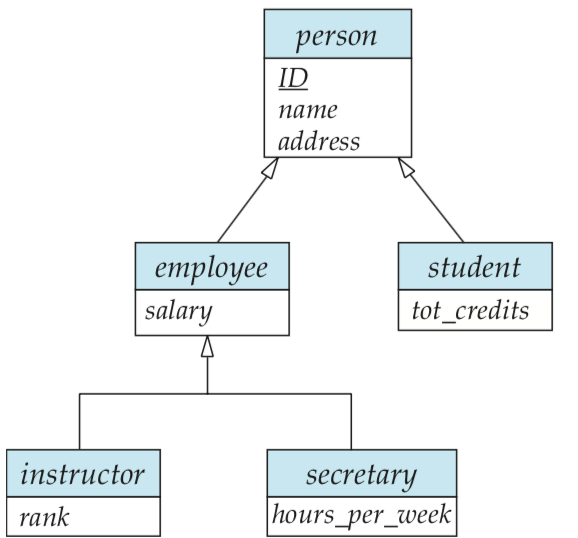
\includegraphics[width=0.35\textwidth]{images/specialization-generalization}
\end{center}

In this case then we would define tables for instructor, secretary, and student.

\end{frame}



\begin{frame}
\frametitle{Generalization and Specialization}

Instructor then created as \textit{(ID, name, address, salary, rank)} with \textit{ID} as the primary key. 

There will be some repetition here as the secretary relation will also have most of the attributes the same, except instead of rank it will have hours per week.

\end{frame}



\begin{frame}
\frametitle{Generalization Alternative}

The alternative representation is to break it up so that we have instructor created as \textit{(ID, rank)}.

This necessitates creating employee as \textit{(ID, salary)}, and person as \textit{(ID, name, address)}. 

This does require a fair amount of repetition in the primary key attribute since it will appear in all tables. 

The primary key is then the only one that is repeated. With foreign keys.


\end{frame}



\begin{frame}
\frametitle{Redundancy}

Both of these things will have some redundancy. 

If the generalization is both disjoint and complete, the first approach is better.

Perhaps the alternative approach is preferable if these two conditions do not hold.

\end{frame}



\begin{frame}
\frametitle{Aggregation}

Aggregation is actually relatively easy to work out. 

The tables for the elements inside the aggregation are created as normal. 

Then the rules for creating the key constraints can just as easily be applied to any relationship that involves the aggregation. 

The primary key of the aggregation is the primary key of its defining set, so just use that. 

No relation is created to specifically represent the aggregation.

\end{frame}



\begin{frame}
\frametitle{Design Decisions}

In creating our E-R diagrams we have implicitly or explicitly made some key design decisions about how we would like to implement the design. 

In some cases there are better choices and worse choices, but in other cases there are alternatives that are equally valid that we could choose between.

\end{frame}



\begin{frame}
\frametitle{Entity vs. Attribute}

A decision we need to make frequently is whether a new piece of data should be added as an attribute or as a new entity. 
 
Let's say we want to add an e-mail address to users.

If the relationship is anything other than 1:1 then it is very unlikely we will choose a new attribute.

\end{frame}



\begin{frame}
\frametitle{Entity vs. Attribute}

How many e-mail addresses are users allowed to have in the system? 

If it is just one, our decision is more interesting. 

If a user can have multiple e-mail addresses, we must choose a new entity to represent e-mails. 

What about letting multiple users share an e-mail address? 

\end{frame}



\begin{frame}
\frametitle{Entity vs. Attribute}

Let's assume that a user can have exactly one e-mail address. 

Then putting it in an attribute is a viable choice. 

What if we put it in another entity? That might not be the best choice here. 

\end{frame}



\begin{frame}
\frametitle{Entity vs. Attribute}

What if instead, we were thinking of adding multiple related fields instead of one field? 

Then it might make more sense to group those things separately in an entity of their own. 

An address, for example, is a number of related fields, street, city, postal code, et cetera. 

If a user has one address we could put all those fields on the user entity, but it might make more sense to move them to a different entity. 

Performance considerations may come into play (eventually) because large entities are unwieldy. 

\end{frame}



\begin{frame}
\frametitle{Entity vs. Attribute}

But the real decision is more philosophical... 

What is an attribute and what is better as a set? 

There is not a bright line between the two and it may depend more on the real-life situation being modelled than any actual technical consideration.


\end{frame}



\begin{frame}
\frametitle{Entity vs. Attribute}

There is a wrong choice, though. 

That is using the primary key of an entity as an attribute of another, instead of a relationship. 

In the E-R diagram it should be represented as a relationshi.

\end{frame}



\begin{frame}
\frametitle{Redundant Attributes}

A common mistake is to write redundant attributes on the relationship. 

If a relationship is drawn between tables $r_{1}$ and $r_{2}$ in the diagram, don't put the primary key of either $r_{1}$ or $r_{2}$ as attributes on that relation.

They are already implied by the fact that there exists a relationship between the two types. 

\end{frame}



\begin{frame}
\frametitle{Entity vs. Relationship}

We are also sometimes faced with the decision about whether to make a particular object an entity or a relationship. 

There are things that are clearly an entity (e.g., a customer)...

... and those that are clearly a relationship (e.g., a shopping cart).

There are other things where it could go either way. 

\end{frame}



\begin{frame}
\frametitle{Entity vs. Relationship}

In an online shopping scenario, though, what about order history? 

This is different from the idea of a shopping cart because if an item changes attributes before purchase, the data in the cart needs to be updated...

If it changes after, for example, the price decreases, it does not change the already-purchased orders.

\end{frame}



\begin{frame}
\frametitle{Entity vs. Relationship}

There are arguments for the relationship approach: it eliminates duplicate data and ensures that if a product is updated then the latest data is shown. 

That might, actually, be an argument for the alternative. 

If a product is purchased then it might make sense to ``freeze'' in place some of its data at the time of purchase (e.g., price).

So it is perhaps advisable to make an entity for a purchase order made. 

\end{frame}



\begin{frame}
\frametitle{Entity vs. Relationship}

Another example in the university schema is what to do with registration? 

When a student takes a class should that be represented by a relation that says the student with the id $x$ registered in the section $y$? 


\begin{center}
	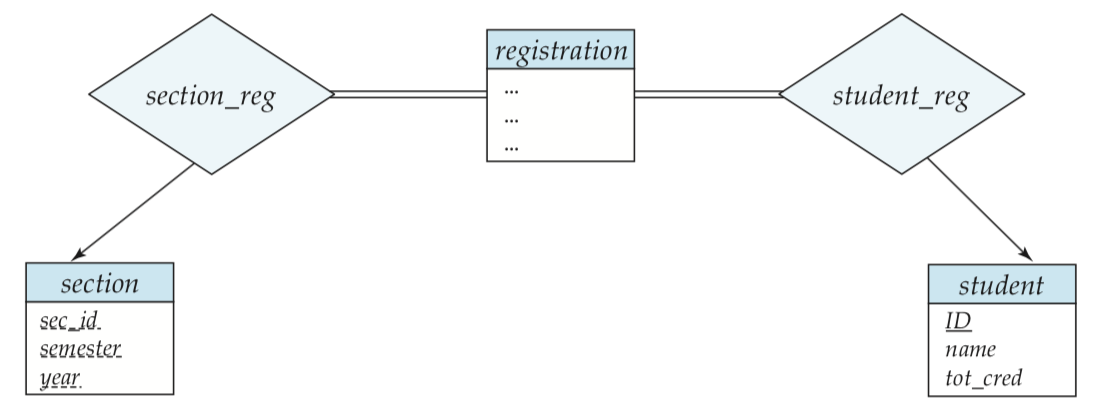
\includegraphics[width=0.7\textwidth]{images/reg-split}
\end{center}

\end{frame}



\begin{frame}
\frametitle{Binary vs. Non-Binary Relationships.}

An $n$-ary relationship can be rewritten as binary.

Consider a work term report: it has an author and an evaluator. 

We could make it a three-way relationship or we could instead break it up into two relationships, or two binary ones.

If it was in one relationship, a work report that has no marker assigned yet would just have \texttt{null} as its assigned value until a marker is assigned.  


\end{frame}



\begin{frame}
\frametitle{Replacing Non-Binary with Binary}

It is always possible to replace an $n$-ary relation with some binary relationships. 

We may need to put an entity in the middle of it to make it all work out.

 Suppose we have a ternary relationship $R$ that connects entities $A$, $B$, and $C$. 
 
 Any attributes of the ternary relationship become an entity $E$. 
 
Three binary relations are created: $R_{A}$ relating $A$ and $E$, $R_{B}$ relating $B$ and $E$, and $R_{C}$ relating $C$ and $E$.


\end{frame}



\begin{frame}
\frametitle{Replacing Non-Binary with Binary}

\begin{center}
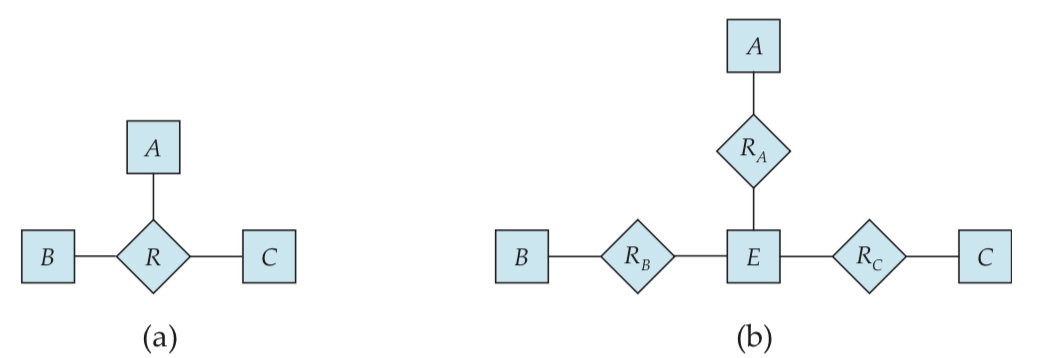
\includegraphics[width=0.9\textwidth]{images/ternary-to-binary}
\end{center}

\end{frame}



\begin{frame}
\frametitle{Don't Do It}

Why we might not split it:

\begin{itemize}
	\item Clarity
	\item Diagram Complexity
	\item Constraints
\end{itemize}

\end{frame}


\begin{frame}
\frametitle{Placement of Attributes}

In the case of one-to-one and one-to-many relationships we could choose to create a table for the relation, but we don't have to... 

We could instead associate the attributes of the relationship with one of the entities. 

If we have a work report entity and we want to relate it to its author, we could have a table that relates the two...

But this wouldn't work for a book and author relationship.

\end{frame}



\begin{frame}
\frametitle{Placement of Attributes}

If an attribute $A$ in the relationship is determined uniquely only by the combination of the entities' identifiers? 

$A$ needs to be placed on that relationship and cannot be put on either side. 

Online shopping with a discount code: the code belongs neither to the customer nor any individual item in the cart.



\end{frame}


\begin{frame}
\frametitle{Think Security!}

Remember, permissions are handed out at the level of the table.

That makes it sometimes necessary to divide some tables so that the appropriate security constraints can be applied. 


\end{frame}


\begin{frame}
\frametitle{Be Normal}

 There are, fortunately, some formal and precise ways for making a determination about whether our designs are appropriate. 
 
 We would like our designs to be ``normal'' and there is a precise definition of what normal is. 


\end{frame}




\end{document}

